In this chapter we are planning the project in general. It is hard to come up with a detailed plan for each sprint now, but this is a rough plan for the whole project. After doing a preliminary study we have made some decisions about methodology tools, technology, collaboration, and a rough project plan. Planning increases the efficiency and it reduces the risks involved. It also facilitates proper coordination within a development team, and this will help us maintain a good control. Planning will help us to achieve our goals by using the available time and resources, and of course planning helps in decision making  

\section{Work breakdown structure}
\label{sec:wbs}
We thoroughly examined the whole project considering the stated scope and the objectives and we were able to decompose it into eight main distinctive modules:

\begin{itemize}
\item Pre-study
\item Requirements elicitation
\item Project planning
\item Application design
\item Application implementation
\item Testing and evaluation
\item Project management
\item Documentation
\end{itemize}

The main modules can be further decomposed into smaller actions. The graphical representation of the whole work breakdown structure can be found in the appendix in chapter \ref{txt:work_breakdown_structure}.

\section{Methodology choice - Scrum}
After fast research and consultation with our mentor and customer(He have experience with CDP student group from last year), we decided to use SCRUM methodology for a few reasons. Requirements and scope of the undertaking were not that precisely defined at the time we had to decide on the methodology. Our approach therefore could not be founded on the sequential methodology as is "waterfall". We wanted to have frequent meetings with our customer and involve him in development process. Sprints in SCRUM allow us just that - 
to have meeting with customer at the end of every sprint, and plan next one together. Sprints does not have to be the same length so we can better managed developing process and risks, and we will be able to have as much sprints as possible under time limit of 13 weeks. SCRUM will give us derivatives that we can enhance in increments and allow us to gradually reduce the risk and keep our customer informed about our progress. SCRUM is also a very popular approach in the software industry, so it is a good choice to learn it.

\section{Organization}
This chapter outlines how the project group is organized and why.
To do our jobs efficiently and effectively it is important to figure out what kind of organizational structure we want. 
Structures provides an overview of who makes decisions and is responsible, how information flows within and between organizational units and suggests what it takes to move between departments. This means that a good organizational structure will give us clarity of the different responsibilitiesy. Since one of our goals is to finish the project in the given time frame, and having a good organizational structure can help us with this, which means it is very important.

\begin{table*}\centering \ra{1.3}
    \caption{Skills and previous experience table. Coding:
        \textcolor{green!100}{$\bullet$} expert,
        \textcolor{green!60}{$\bullet$} experienced,
        \textcolor{yellow!75}{$\bullet$} neutral,
        \textcolor{orange!90}{$\bullet$} little experience,
        \textcolor{red!80}{$\bullet$} no experience}
    \label{tab:skills}
    \vspace{2mm}
    \begin{tabular}{lcccc}
    \toprule
                                & Agnethe   & Tomas & Milos & Jan \\
    \midrule
    \textbf{Leadership                 } & \colorB & \colorE & \colorD & \colorC \\ 
    \textbf{Scrum                      } & \colorB & \colorE & \colorE & \colorE \\ 
    \textbf{Mobile software development} & \colorC & \colorE & \colorB & \colorE \\ 
    \textbf{\LaTeX                     } & \colorE & \colorB & \colorE & \colorB \\ 
    \textbf{Network programming        } & \colorD & \colorC & \colorC & \colorC \\ 
    \textbf{Image processing           } & \colorE & \colorC & \colorE & \colorD \\ 
    \textbf{Java                       } & \colorC & \colorD & \colorA & \colorE \\ 
    \textbf{C++                        } & \colorE & \colorB & \colorC & \colorB \\ 
    \textbf{Testing                    } & \colorE & \colorB & \colorD & \colorC \\
    \bottomrule
    \end{tabular}
\end{table*}

\subsection{Role Assignment}
To assign roles according to our skills and previous experience we have decided to make a survey of relevant knowledge. 
Results of this survey can be seen in table \ref{tab:skills}. 
This table was used as a base for our role assignment.
In the beginning, during planning, we did not establish so many roles, but during the development process itself we found out that some of them are necessary. 
Nevertheless we use only few roles and the responsibility of unused roles (mention in compendium) are distributed to all members. 
We decided to embrace this as a development team were we are all equal.
The assigned roles can be seen in table \ref{tab:roles}. 

\begin{table*}\centering \ra{1.3}
    \caption{Assigned roles and their responsibilities}
    \label{tab:roles}
    \vspace{2mm}
    \begin{tabularx}{\textwidth}{llX}
    \toprule
    Role    & Person   & Responsibility \\
    \midrule
    \textbf{Project Leader}             & Agnethe &
        Responsible for progress of the project according to the plan.
        Distributes work to group members.
        Has final call in arguments.\\
    \textbf{System Architect}             & Milos &
        Check consistency and analyze all layers of the product. \\
    \textbf{Scrum Master}             & Agnethe &
        Leads the scrum stand-ups. \\
    \textbf{Communication Responsible}  & Jan &
        Responsible for communicating with customer and supervisor.
        Regularly send meeting minutes, agenda and other documents to customer and supervisor. \\ 
    \textbf{QA Responsible} & Tomas &
        Ensure a quality of all documents and end-product.        \\ 
    \textbf{Documentation Responsible} & Agnethe &
        Responsible for delegating and supervising work on final report.        \\         
    \bottomrule
    \end{tabularx}
\end{table*}

\section{Risk Management}
In the table \ref{tab:risks} the consequence and possibility in a number between 1-10. The risk, or the riskfactor, is the consequence multiplied with the possibility. The risks in this table is very obvious ones. 

Other risks we can see from analyzing the skill table. If for example the only two persons on the team who are familiar with image processing is away, then this will be a risk. There is a great possibility that this kind of task will take longer time then planned for. 

Also if some of the rows in the skill table all were painted red, which would imply that the team had experience with this, then this would be a risk. In such a case, we would have to talk to our customer and consider scaling down this task. 
\ref{tab:risks}

\begin{sidewaystable}
    \caption{Handling risks}
    \label{tab:risks}
    
    \centering \ra{1.3}
    \vspace{2mm} %\rotatebox{90}{
    \begin{tabularx}{500pt}{XcccXX}
    \toprule
        Event & Consequence & Possibility & Risk  & Reactive Measures & Proactive Measures \\
    \midrule
Someone gets sick & 4     & 5     & 20    & Other people do more work.  & Free weekends \\
Coding problems & 4     & 7     & 28    & Talk to supervisor \& Guru office & preparing for the task \\
Testing problems & 4     & 4     & 16    & Talk to customer about reformulating requirements & Double check requirements with customer \\
Implementing things we are not supposed to & 7     & 6     & 42    & Try to adopt functionality or start all over & Don't do anything that is not in backlog and keep good communication with customer \\
Dead end with technologies & 8     & 8     & 64    & Talk to supervisor \& Guru office & Do thoroughly research \\
Unrealistic time estimate & 7     & 8     & 56    & Work overtime  & Planing poker \\
Frequent changes in requirements specification & 6     & 3     & 18    & Renegotiate with a customer & Try no to change finished modules and keep weekly meetings with the customer \\
Customer too ambitious & 9     & 5     & 45    & Renegotiate with a customer & Keep customer informed about what  to expect \\
Hardware problems & 9     & 3     & 27    & Obtain a new one & Keep your devices updated \\
\bottomrule
\end{tabularx}
\end{sidewaystable}
\subsection{Limitations}
\label{sec:limitations}
We are developing this project under a few technical, resource, time and knowledge limitations. 

Our biggest limitation is the image processing part. Half of the team has no experience with this, and the other half has little experience. Their experience is mostly theoretical information about the subject, and practical experience is preferred. We are aware of this limitation, and our plan is to learn by doing. We are going to start developing, and teach ourself while coding. We chose this approach because we do not want to spend more time than necessary doing research.

Another limitation is lack of experience with Mobile development within the development team. All of the team members have Android phones, and to be able to test our application, we have to develop an Android application. Only one team member have experience with this. 

If we are not scaling down the project, then we do not have all necessary resources to test the system. As an example we do not have a huge audience. Also  we do not have access to a big screen etc. This is also a limitation.  

As this course last for a 13 weeks, it is normal that we have to make some trade-offs.
This project is technically difficult, and there is a limited amount of time. 


\section{Communication}
Specific guidelines and practices were adopted
so that the team and the customer could continuously verify that the project development keeps the right direction and that the requirements are being fulfilled.

\subsection{Customer collaboration}
Since the scope of the project and the actual requirements are determined by the customer it is essential to establish tight collaboration practices and even involve the customer in the collaboration tools the team uses. In the next paragraph the main means utilized for interaction with the customer are listed. 

\paragraph{Meetings}
We agreed on holding the weekly meetings taking approximately 60 minutes. The standard agenda consists of the approval of the meeting minutes summarizing the last meeting, comments on the meeting minutes and the specific issues regarding the team-customer collaboration and technical issues. As the customer is located in Oslo the meetings will be carried out using the video-conference devices provided by the NTNU (accessible in the Accenture Lab) and Skype software. Contents of each meeting including the topics discussed, decisions made and the future plans are summarized in the meeting minutes. The team should provide the customer with the meeting minutes document before the next meeting is held.

\paragraph{Email}
Standard email messages will also serve the purpose of the communication mean, both team and the customer agreed on responding to the queries as soon as possible.

\paragraph{Documents}
In order to provide the customer with the convenient overview of the work done all relevant documents including the meeting minutes, private notes taken during the meetings and the project report are stored on the Google drive cloud storage service and shared with the customer.

\paragraph{Other tools}
As mentioned earlier the team decided to utilize the Target Process 3 as a collaboration tool suitable for handling Scrum-driven projects. The customer was invited to join the framework so that he could observe the development process more closely. Thanks to the software tool the customer is able to easily adjust the order of the user stories according to his preferences.

\subsection{Team collaboration}
Mostly during the pre-study phase the developers need to distribute and maintain the information considered important for the next work. The Facebook group was chosen and set up to serve this purpose as it disposes of the tools suitable for exchanging website links, opinions and multimedia.

It has been also decided that the project report should be written continuously by all members as a part of our daily workflow. Through this practice the team will be able to keep track of the amount of work done and all members will make sure they understand well what direction the project is aiming.

\section{Duration and workload}
Compendium proposed week workload 25 person-hours per week. 
During our internal meeting we have decided that each member will spend 30 hours per week because our team consists only of 4 members. 
We agreed on fixed daily working hours so that we could distribute the workload through the whole semester.
We will do daily stand-ups according to Scrum methodology.

According to work break down structure \ref{sec:wbs} and presented week workload, there was created initial time estimation of whole project. 
You can see the estimation in table \ref{tab:initial-time-estimation}. 
As a part of a evaluation, spent hours will be filled, and then retrospective to the planning phase can be done.

\begin{table*}[!h]
	\caption{Initial time estimation table}
	\label{tab:initial-time-estimation}
	\def\arraystretch{1.25}
	\begin{tabularx}{\textwidth}{Xcccc}
		\toprule[1mm]
		\multirow{2}{*}{\textbf{Task}} &
		\multirow{2}{*}{\textbf{From date}} & 
		\multirow{2}{*}{\textbf{To date}} & 
		\multicolumn{2}{c}{\textbf{Hours}} \\
 				& & & \textbf{Estim.} & \textbf{Spent} \\
		\midrule
		Pre-study 					& 26.08.2013 & 15.09.2013 & 70 &  ?\\
		Requirements elicitation 	& 26.08.2013 & 29.09.2013 & 80 &  ?\\
		Project planning			& 26.08.2013 & 15.09.2013 &	75 &  ?\\
		Application design 			& 26.08.2013 & 27.10.2013 & 90 &  ?\\
		Application implementation	& 02.09.2013 & 20.11.2013 &	450 &  ?\\
		Testing and evaluation 		& 02.09.2013 & 20.11.2013 & 130 &	?\\
		Project Management  		& 26.08.2013 & 20.11.2013 & 120 &  ?\\
		Documentation				& 26.08.2013 & 20.11.2013 &	425 &  ?\\
		\midrule		
		\textbf{$\sum$}	& &	&		1440	& \textbf{?} \\								
		\bottomrule[1mm]
	\end{tabularx}
\end{table*}


\section{Project scope}
After third meeting with our customer we decided to lay out the scope of the project that is tangible and doable under 13 weeks. Customer idea although good and innovative has one flaw - it is a huge undertaking!

As we operate under certain limitations we explained in \ref{sec:limitations}, we agreed with customer on next terms:
\begin{itemize}
	\item Take project title as domain of work and not final product.
	\item Scale down problem but attack all main problems of the domain.
	\item When designing architecture disregard scaling of product.
	\item Disregard some of problems that are not important for final prototype, but  with approval of a customer before making this kind of decision.
\end{itemize}

\section{Project plan}
This section contains a general plan for all the sprints, the general sprint duration, and all the milestones for this project. In this chapter there is also a gantt diagram and a work breakdown structure to visualize how we plan to reach the different milestones.

\subsection{General plan for the sprints}

In general the sprints will last for two weeks. The only sprints that does not have that length, is the first and the last. This is because these two are more related to getting started, and finishing the project. The other sprints will have a more general approach. 

After each sprint we have a sprint review with the customer. The sprint reviews takes place every other Thursday, which means that the Wednesday before, the team has to prepare for the review. In each sprint review we both present and demonstrate what we have done so far. After the presentation we are doing a retrospective with the customer. It is important to evaluate our sprint delivery the customer. After the retrospective we will plan the next sprint, and now the customer can prioritize which user stories he wants us to work on next. The Friday after the sprint review, the team will do a detailed planning of the next sprint. 

On the Thursdays in between we have weekly meetings with the customer. It is important to have good communication with the customer. These meetings gives us opportunities to ask questions, and to make sure that we are on the right track.

You can see detailed sprint decomposition in figure \ref{img:sprint_detail}.

\begin{figure}[!ht]
    \begin{center}
    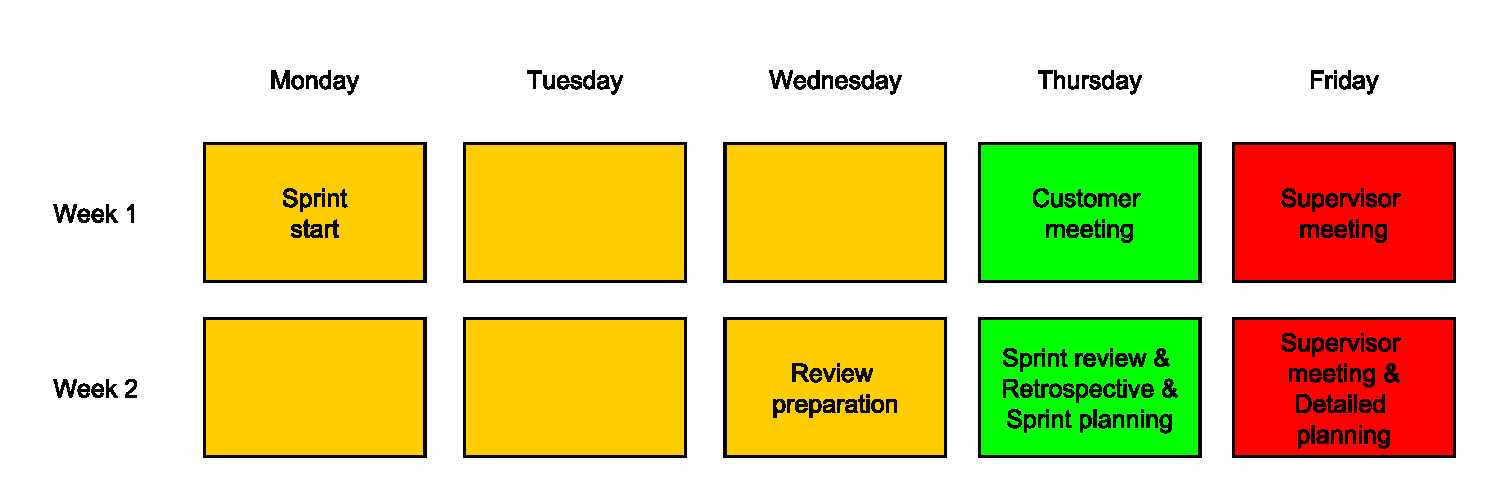
\includegraphics[scale=0.5]{images/sprint_detail.eps}
    \caption{Diagram depicting detailed sprint decomposition.}
    \label{img:sprint_detail}
    \end{center}
\end{figure}

\paragraph{Sprint duration:}
Sprint 0 (ends 6th of September)
Sprint 1 (ends 20th of September)
Sprint 2 (ends 4th of October)
Sprint 3 (ends 18th of October)
Sprint 4 (ends 1st of November)
Sprint 5 (ends 15th of November)


\subsection{Product Milestones}

We set milestones in order to more accurately ascertain whether or not the project is on schedule. After finishing some group of the milestones we will have running prototypes (Deliverables). There are 4 prototypes in total we 
agreed on. After reaching point of 4 prototypes we will have meeting with our customer about how the project is about to continue. The 3th prototype implies that all milestones are reached. 
Although the order of prototypes may look like a waterfall approach that is not the case.
Overview of all milestones and 4 prototypes (Deliverables).

\paragraph{Obedient client  - Prototype 1}
\begin{itemize}
	\item Put "Hello World" project to gitHub and pull it to every group member's local storage.
	\item Set up protocol for client \& server.
	\item Make server able to listen for clients.
	\item One client connects to the server.
	\item The server sends command to one client.
	\item The client receives one command.
	\item The client "plays" one command (white light 10 seconds).
\end{itemize}

\paragraph{Obedient crowd - Prototype 2}
\begin{itemize}
	\item Multiple clients connect to the server.
	\item The server sends same signal to multiple clients.
	\item The server sends multiple different commands to the client.
	\item The client plays commands (Red light 2 seconds, Green light 2 seconds).
\end{itemize}

\paragraph{Traffic light control - Prototype 3}
\begin{itemize}
	\item Server identifies one client from light.
	\item Server maps one client to grid (4 quads).
\end{itemize}

\paragraph{Digital lighter stone age - Prototype 4}
\begin{itemize}
	\item Server identifies multiple clients from light.
	\item Server maps all devices to the grid.
	\item Server play whole picture to the grid.
\end{itemize}


\begin{itemize}
	\item Finish of Project Plan document.
	\item Learn about team dynamics.
\end{itemize}

\section{Gantt diagram}
You can see the Gantt chart in figure \ref{fig:gantt}.
\begin{figure}
    \begin{center}
        \label{fig:gantt}
        \caption{Gantt Chart: Allocation of sprints into weeks.}
        \begin{sideways}
            \begin{gantt}{9}{14}
                \begin{ganttitle}
                   \titleelement{Week}{14}
                \end{ganttitle}
                \begin{ganttitle}
                   \titleelement{1}{1}
                   \titleelement{2}{1}
                   \titleelement{3}{1}
                   \titleelement{4}{1}
                   \titleelement{5}{1}
                   \titleelement{6}{1}
                   \titleelement{7}{1}
                   \titleelement{8}{1}
                   \titleelement{9}{1}
                   \titleelement{10}{1}
                   \titleelement{11}{1}
                   \titleelement{12}{1}
                   \titleelement{13}{1}
                   \titleelement{14}{1}
                \end{ganttitle}
                \ganttbar{Sprint 0}{0.5}{1.5}
                \ganttbarcon{Sprint 1}{2}{2}
                \ganttbarcon{Sprint 2}{4}{2}
                \ganttbarcon{Sprint 3}{6}{2}
                \ganttbarcon{Sprint 4}{8}{2}
                \ganttbarcon{Sprint 5}{10}{2}
                \ganttbarcon{Sprint 6}{12}{1.5}
            \end{gantt}
        \end{sideways}
    \end{center}
\end{figure}


\section{Test plan}
The purpose of this chapter is to introduce the overall plan for the testing of our product, and it describes the scope of the overall testing.
In this chapter we will explain how we plan to test our product, who will be responsible for it, and very short mention the test criteria.
This is the strategy that will be used to verify and ensure that the product meets its requirements, and of course the quality attributes. 

\subsection{Approach}
This is a proof of concept project. The customer did not want us to focus on the testing. We are focusing on the happy path. A happy path is a default scenario featuring no exceptional or error conditions, and comprises the sequence of activities executed if everything goes as expected. Happy path testing is a well-defined test case that uses known input, that executes without exception and that produces an expected output. This means that we do not spend time actually writing tests, but still we have to manually test that the product does what it is supposed to.

We manually have to test the integration between the sprints, and we have do this continuously to ensure that the modules of the various sprints are well integrated. We are also doing verification and validation testing. This is the process of checking that the product meets specifications and that it fulfills its intended purpose. It may also be referred to as software quality control, and it is high-level checking. Again we do this manually, which means we do not write tests for this. We will write about these tests in each of the sprint chapters. 


\subsection{Responsibilities}
The whole development team is responsible for testing the product. 
Each person is responsible for testing their own code. It is important to perform continuously testing. We also plan to have someone different to test, rather than the person who wrote the specific code segment. 
This is mostly for the usability of the product.As we are short on manpower and time we can not guarantee that this is always the case.
Testing will be done continuously through out the sprints, when the relevant functionality is implemented, and they will be performed at a time that allows the developers to fix bugs before the sprint has ended. 

\subsection{Test criteria} 
A test is considered passed when it achieves the expected result.
A test will be considered to have failed if the result differs from what was expected.

TODO: WRITE CRITERA

\subsection{Measurement of Project Successes}
To measure success of our end-product we have to use the test criteria and see if the critera is fulfilled. The product should function according to customer's requirements.

